% Copyright 2016 Jochen Kursawe. See the LICENSE file at the top-level directory 
% of this distribution and at https://github.com/kursawe/MCSTracker/blob/master/LICENSE.
\documentclass[a4paper,11pt]{article}

\usepackage{amsmath}
\usepackage{amssymb}
\usepackage{textcomp}
\usepackage{fullpage}
\usepackage{graphicx}
\usepackage{subfigure}
\usepackage{lmodern}
\usepackage[hidelinks]{hyperref}
\usepackage{url}
\usepackage{soul}
\usepackage{afterpage}
\usepackage{algorithm2e}
\usepackage{enumitem}

\newcommand{\Drosophila}{\textit{Drosophila}~}
\newcommand{\insilico}{\textit{in silico}~}
\newcommand{\invivo}{\textit{in vivo}~}
\newcommand{\invitro}{\textit{in vitro}~}
\newcommand{\todo}[1]{{\color{red} \bf TODO: #1}}
\newcommand{\comp}[1]{\texttt{#1}}
\newcommand{\comment}[1]{{\color{red} [#1]}}
\usepackage{cite}

% for doi formatting
\usepackage{doi}
\renewcommand\doitext{}

% editorial packages
\usepackage{color}
\usepackage{lineno}
\usepackage{setspace}
\usepackage{xcolor}

\newcommand{\jochen}[1]{\textbf{\textcolor{red}{#1}}}
\newcommand{\alex}[1]{\textbf{\textcolor{blue}{#1}}}

%\parindent 0pt
\title{Cell tracking paper}

%%%%%%%%%%%%%%%%%%%%%%%%%%%%%%%%%%%%%%%%%%%%%%%%%%%%%%%%%%%%%%%%%
%%%%%%%%%%%%%%%%%%%%%%%%%%%%%%%%%%%%%%%%%%%%%%%%%%%%%%%%%%%%%%%%%

\begin{document}

%% For manuscript editing only, remove for final version
%\modulolinenumbers[5]
\linenumbers
\doublespacing

\begin{flushleft}
{\Large {\bf Robust cell tracking in epithelial tissues through identification of maximum common subgraphs}}
\vspace{1.0em}

Jochen Kursawe$^{1,\ast}$, 
R\'{e}mi Bardenet$^{2}$,
Jeremiah J. Zartman$^{3}$,
Ruth E. Baker$^{1}$,
Alexander G. Fletcher$^{4,5,\ast}$ 
\vspace{1.0em}

$^{1}$ Mathematical Institute, University of Oxford, Andrew Wiles Building, Radcliffe Observatory Quarter, Woodstock Road, Oxford, OX2 6GG, UK
\\
$^{2}$ CNRS \& CRIStAL, Universit\'{e} de Lille, 59651 Villeneuve d'Ascq, France
\\
$^{3}$ Department of Chemical and Biomolecular Engineering, University of Notre Dame, 182 Fitzpatrick Hall, Notre Dame, IN 46556, USA \\
$^{4}$ School of Mathematics and Statistics, University of Sheffield, Hicks Building, Hounsfield Road, Sheffield, S3 7RH, UK \\
$^{5}$ Bateson Centre, University of Sheffield, Sheffield, S10 2TN, UK
\vspace{1.0em}

$^{\ast}$ E-mail: kursawe@maths.ox.ac.uk, a.g.fletcher@sheffield.ac.uk
\end{flushleft}

\date{\today}
\vspace{1.0em}

%%%%%%%%%%%%%%%%%%%%%%%%%%%%%%%%%%%%%%%%%%%%%%%%%%%%%%%%%%%%%%%%%

%\noindent \textbf{Word count:} 7932 
%\vspace{1.0em}

%%%%%%%%%%%%%%%%%%%%%%%%%%%%%%%%%%%%%%%%%%%%%%%%%%%%%%%%%%%%%%%%%

\noindent \textbf{Data accessibility:} The datasets and code supporting this article are publicly available under \texttt{https://github.com/kursawe/MCSTracker}.
\vspace{1.0em}

%%%%%%%%%%%%%%%%%%%%%%%%%%%%%%%%%%%%%%%%%%%%%%%%%%%%%%%%%%%%%%%%%

\noindent \textbf{Competing interests:} We have no competing interests.
\vspace{1.0em}

%%%%%%%%%%%%%%%%%%%%%%%%%%%%%%%%%%%%%%%%%%%%%%%%%%%%%%%%%%%%%%%%%

\noindent \textbf{Authors' contributions:} 
%All submissions, other than those with a single author, must include an Authors’ Contributions section which individually lists the specific contribution of each author. The list of authors should meet all of the following criteria; 1) substantial contributions to conception and design, or acquisition of data, or analysis and interpretation of data; 2) drafting the article or revising it critically for important intellectual content; and 3) final approval of the version to be published.
JK, RB, JJZ, REB, and AGF conceived the study and contributed to the manuscript. JK developed the algorithm and carried out the data segmentation and performance analysis. JK, REB, and AGF drafted the manuscript. JJZ provided microscopy data. All authors gave final approval for publication. 
\vspace{1.0em}
%%%%%%%%%%%%%%%%%%%%%%%%%%%%%%%%%%%%%%%%%%%%%%%%%%%%%%%%%%%%%%%%%

\noindent \textbf{Keywords:} Cell tracking, planar graphs, maximum common subgraph, epithelial sheets

%\todo{reconsider the use of the terms `network' and `graph'.}

%%%%%%%%%%%%%%%%%%%%%%%%%%%%%%%%%%%%%%%%%%%%%%%%%%%%%%%%%%%%%%%%%
%%%%%%%%%%%%%%%%%%%%%%%%%%%%%%%%%%%%%%%%%%%%%%%%%%%%%%%%%%%%%%%%%

\clearpage

\section*{Abstract}
% <=200 words
Tracking of cells in live-imaging microscopy videos of epithelial sheets is a powerful tool for investigating fundamental processes in embryonic development. 
Observing the growth, proliferation, intercalation, and apoptosis of individual cells helps us understand how global morphogenetic processes, such as tissue invagination or extension, are locally regulated and controlled. 
Accurate cell tracking requires correctly resolving cells moving in and out of field of view between frames, cell neighbour exchanges, cell removal and cell division events. 
Here, we present a novel algorithm for epithelial cell tracking. 
The algorithm exploits the graph-theoretic concept of a `maximum common subgraph' to track cells between successive frames of a video. 
It does not require the adjustment of tissue-specific parameters, and scales in polyonomial time with tissue size. 
The algorithm does not rely on precise positional information and thus permits large cell movements between frames, enabling cell tracking in data sets acquired at low temporal resolution due to experimental constraints such as photoxicity. 

%%%%%%%%%%%%%%%%%%%%%%%%%%%%%%%%%%%%%%%%%%%%%%%%%%%%%%%%%%%%%%%%%
%%%%%%%%%%%%%%%%%%%%%%%%%%%%%%%%%%%%%%%%%%%%%%%%%%%%%%%%%%%%%%%%%

\clearpage

\section{Introduction}

Live-imaging microscopy is a powerful, and increasingly quantitative, tool for gaining insight into fundamental processes during embryonic development~\cite{Stephens2003, Pantazis2014, Truong2011}. Quantitative information on cell growth, proliferation, death, shape changes and movement extracted from live-imaging reveals how such processes are regulated to give correct tissue-level behaviour. This approach has been particularly successful in characterising the growth and patterning of embryonic epithelial tissues in a number of model organisms~\cite{Mao2011, Gibson2006, Rauzi2008, Collinet2015, Ritsma2014,Parker2006}. 

A common experimental technique for visualising cell shapes in an epithelial sheet is to fluorescently tag a binding molecule, such as E-cadherin (figure~\ref{fig:data}A). 
The analysis of time-lapse microscopy data obtained from such tissues is extremely challenging \cite{Pantazis2014, Truong2011}, especially in cases of imaging data of rapidly evolving tissues, and when limitations of, for example, microscope speed, imaging resolution or phototoxicity inhibit the creation of datasets with high temporal and spatial resolution.

%%%%%%%%%%%%%%%%%%%%%%%%%%%%

\begin{figure}[h]
\centering
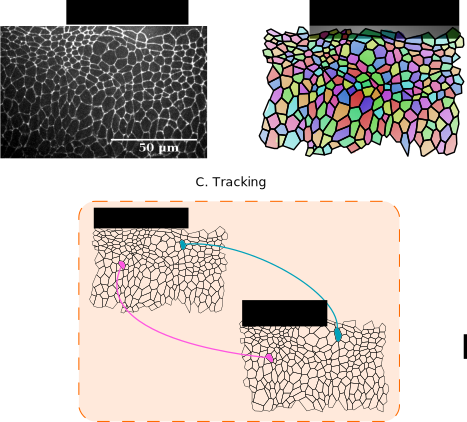
\includegraphics{Figures/Data_figure/Data_figure.pdf}
\caption{Pipeline for analysing epithelial tissues. 
(A) Example raw data. 
Frame of a live-imaging microscopy video of the lateral epidermis of a stage-eleven \Drosophila embryo, expressing DE-Cadherin::GFP. 
See Experimental Methods for details. 
(B) Segmentation of this image, showing cell shapes (coloured regions) and polygonal approximation based on three-cell junctions (black lines). See Methods section for details of segmentation. 
(C) Cell tracking involves registering individual cells across consecutive segmented images.} 
\label{fig:data}
\end{figure}

%%%%%%%%%%%%%%%%%%%%%%%%%%%%


The analysis of time-lapse microscopy data comprises two major steps: segmentation and tracking (registration). Segmentation must be performed for each frame of a video and involves the identification of objects and landmarks, such as cell shapes (figure~\ref{fig:data}B). 
Automated segmentation is hindered by various factors such as noise in fluorescent signals, uneven illumination of the sample, or overlapping cells in a two-dimensional projection. 
Often, manual correction is necessary to address over-segmentation, where too many cells are detected, or under-segmentation, where too few cells are detected~\cite{Mashburn2012, Cilla2015, Schiegg2013}. 
Tracking involves the association of segmented cells across video frames (figure~\ref{fig:data}C) and requires resolving cellular movement, cell division, cell death, and cells entering and leaving the field of view~\cite{Schiegg2013}.

Numerous algorithms are available for the segmentation and tracking of cellular-resolution microscopy data~\cite{Mashburn2012,Cilla2015,Heller2016}. 
Common methods for cell tracking utilize optimization techniques to minimise differences in cellular properties between two frames~\cite{Padfield2011, Cilla2015, Youssef2011, Wait2014, Winter2011}. 
The min-cost max-flow algorithm~\cite{Padfield2011} uses linear integer programming to minimise differences in cell areas, perimeters, orientations, and locations between frames, whereas multiple-parameter tracking \cite{Youssef2011} employs global optimization to minimize differences in cell shapes as well as locations. 
In contrast, multitemporal association tracking~\cite{Wait2014,Winter2011} minimises differences in cell locations and sizes by using a probabilistic approach that finds the most likely extension to existing cell trajectories. 
Chain-graph models~\cite{Sommer2011} minimise differences in cell velocity while overcoming mis-segmentation by verifying that each segmented object continues or begins a cell trajectory in successive frames. 
Optical flow (`warping') between successive frames can be used to guide cell tracking as well as segmentation~\cite{Liu2014}.
It is also possible to combine segmentation and tracking of 2D microscopy videos by interpreting time as a third spatial dimension and employing 3D segmentation techniques~\cite{Bellaiche2011}. 

The nearest-neighbour method associates two cells in consecutive frames with each other if their respective centroids have minimal distance within the field of view~\cite{Mashburn2012}, or if their overlap in pixels within the field of view is maximal~\cite{Aly2014, Wang2010}. 
Particle image velocimetry, a technique originally developed to analyse fluid flow~\cite{Raffel2007}, has also been employed to track cells in epithelial tissues \cite{Puliafito2012}. 

Software implementations and computational tools for cell tracking include FARSIGHT~\cite{Kofahi2010} (segmentation only), SeedWaterSegmenter~\cite{Mashburn2012} (nearest-neighbour tracking), ilastik~\cite{Sommer2011} (chain-graph models), Tufts Tissue Tracker~\cite{Cilla2015} (min-cost max-flow algorithm), Tracking with Gaussian Mixture Models \cite{Amat2014} (nearest-neighbour tracking), Packing Analyzer~\cite{Aigouy2010} (particle image velocimetry) and EpiTools \cite{Heller2016} (nearest-neighbour tracking).  
These algorithms and software tools primarily rely on there being small differences in cell positions and shapes across consecutive images. 
Their performance is therefore hindered when analysing data from \invivo studies where phototoxicity provides a barrier to high temporal resolution imaging \cite{Hoebe2007,Wood2005,Mavrakis2008}. 
To address this limitation, we propose a novel algorithm for cell tracking that uses only the connectivity of cell apical surfaces (figure~\ref{fig:data}). 
By representing the cell sheet as a physical network in which each pair of adjacent cells shares an edge, we show that cells can be tracked between successive frames by finding the \textit{maximum common subgraph} (MCS) of the two networks: the largest network of connected cells that is contained in these two consecutive frames. 
It is then possible to track any remaining cells based on their adjacency to cells tracked using the MCS.
Our algorithm does not require the tuning of parameters to a specific application, and scales in subquadratic time with the number of cells in the sheet, making it amenable to the analysis of large tissues. 

We demonstrate here that our algorithm resolves tissue movements, cell neighbour exchanges, cell division, and cell removal (for example, by delamination, extrusion, or death) in a large number of \insilico data sets, and successfully tracks cells across sample segmented frames from \invivo microscopy data. The remainder of the paper is structured as follows. 
In Section~\ref{sec:methods} we describe the technical details. 
In Section~\ref{sec:results} we analyse the performance of the algorithm on \insilico and \invivo datasets. 
Finally, in Section~\ref{sec:discussion} we discuss future extensions and potential applications.

%%%%%%%%%%%%%%%%%%%%%%%%%%%%%%%%%%%%%%%%%%%%%%%%%%%%%%%%%%%%%%%%%
%%%%%%%%%%%%%%%%%%%%%%%%%%%%%%%%%%%%%%%%%%%%%%%%%%%%%%%%%%%%%%%%%

\section{Methods}
\label{sec:methods}

We begin with a conceptual overview of our cell tracking algorithm; a detailed description of each step of the algorithm is provided in the section `\ref{sec:mathematical_formulation} Mathematical formulation'.
The input to the algorithm is a set of segmented images obtained from a live-imaging microscopy data set of the apical surface of an epithelial cell sheet. 
For each image, the segmentation is assumed to have correctly identified which cells are adjacent and the locations of junctions where three or more cells meet. This information is used to generate a polygonal approximation to the cell tessellation (figure~\ref{fig:data}B-C). 
The statistics of polygonal approximations are commonly used to characterise and explore morphological processes in epithelial tissues~\cite{Farhadifar2007, Cilla2015, Escudero2011, Sanchez-Gutierrez2015,Saez2013}. 

Our algorithm tracks cells between each pair of consecutive images in three steps (figure~\ref{fig:methods}). 
First, we use a MCS-approach \cite{Ullmann1976,Krissinel2004} to generate an initial bijection between the two images that includes every cell whose connections to its neighbours do not change between images, e.g. due to cell rearrangements (figure \ref{fig:methods}B). 
Second, we remove from the bijection any cells that have less than three isolated connections to other cells in the MCS (figure~\ref{fig:methods}B-C), since these cells are likely to have been matched incorrectly.
Third, we extend the MCS to track any remaining cells that were not included in the bijection and we  identify cell division and `removal' (delamination, extrusion or death) events (figure~\ref{fig:methods}D) through characteristic changes to the local cell network under these events.

%%%%%%%%%%%%%%%%%%%%%%%%%%%%
\begin{figure}[ht!]
\centering
\includegraphics{Figures/algorithm_intro/algorithm_intro_on_data.pdf}
\caption{Illustration of our cell tracking algorithm. 
(A) Two consecutive segmented time-lapse images (left and right columns) of the lateral epidermis of a stage-eleven \Drosophila embryo, taken five minutes apart. 
See Experimental Methods for details.
There are several cell neighbour exchanges between these images. 
(B) We first identify a cell mapping between the two graphs based on the conserved MCS. 
This includes correctly tracked (green/light) cells and weakly connected cells (purple/dark). 
Here, the conserved MCS incorrectly tracks two cells (yellow/light dots). 
(C) Weakly connected cells are removed from the conserved MCS to prevent mismatches. 
(D) An extended tracking mapping is constructed, which includes more cells. 
See Methods section for details. 
The remaining white cells enter or leave the frame of view between images and therefore are not tracked.}
\label{fig:methods}
\end{figure}

%%%%%%%%%%%%%%%%%%%%%%%%%%%%

In the first of the three steps shown in figure~\ref{fig:methods}, the MCS is constructed by iterative extension from an initial seed. 
The technical details of this iterative extension are described below.
Briefly, this initial seed is found by identifying two cells in consecutive images whose neighbourhoods have identical graph structures.
The full MCS is then constructed by iteratively adding cells after inspecting MCSs of the cells' extended neighbourhoods. 

%%%%%%%%%%%%%%%%%%%%%%%%%%%%%%%%%%%%%%%%%%%%%%%%%%%%%%%%%%%%%%%%%

\subsection{Mathematical formulation}
\label{sec:mathematical_formulation}

\paragraph{Preliminaries}

We begin by introducing the graph theoretic terminology and notation~\cite{Wilson2010} used to describe our algorithm. 
%We define MCSs in the context of epithelial sheet microscopy data. 
We consider each pair of successive segmented images as vertex-labelled graphs\footnote{A \textit{graph} is an ordered pair $G = (V, E)$, where $V \subseteq \mathbb{N}$ and $E \subseteq \{ A \subseteq V : |A| = 2 \}$. 
The elements of $V$ and $E$ are called the \textit{vertices} and \textit{edges} of $G$, respectively. Given a graph $G = (V,E)$, a \textit{vertex labelling} is a function of $V$ to a set of labels. With this function, $G$ is called a \textit{vertex-labelled} graph.} $G = (V, E)$ and $G' = (V', E')$, respectively. 
Here and throughout, we use a prime symbol $^\prime$ to refer to the latter of the consecutive images.
Each vertex in $G$ or $G'$ corresponds to one cell in the respective segmentation, and two vertices share an edge in the graph if the corresponding cells are adjacent.
Throughout, we assume the graphs $G$ and $G'$ to be simple, planar and connected; we emphasise that these graphs represent the dual of the polygonal cell packing (figure \ref{fig:mcs_construction}A).
% * <remi.bardenet@gmail.com> 2016-03-27T20:52:11.630Z:
%
% The graph given by the contours of the cells in an image can clearly be assumed to be planar, simple, and connected. You're defining G as the dual of this graph, and implicitely using graph-theoretic results that guarantee G is planar, simple and connected. It would be clearer to state them explicitely.
%
% response: edited the sentence above to clarify this.
%
% ^ <remi.bardenet@gmail.com> 2016-03-27T21:02:28.888Z:
%
% and you should give a good reference for the graph notions.
%
% response: We currently cite \cite{Wilson2010} for this (reference 34), see first sentence of the mathematical formulation. Let me know if you think we need an additional/different reference.
%
% ^.
These assumptions are reasonable in the case of simple epithelial cell sheets.

%%%%%%%%%%%%%%%%%%%%%%%%%%%%

\begin{figure}[ht!]
\centering
\includegraphics{Figures/initial_mapping_figure/mcs_construction.pdf}
\caption{Construction of the MCS. 
(A) Overlay of a polygonal tessellation (grey) and the corresponding cell network (black). Each cell corresponds to one vertex in the network, and two vertices share an edge if the corresponding cells are adjacent. The network of cells is used by the algorithm to determine the MCS between tessellations corresponding to consecutive time frames in a microscopy video. Note that the network degree of a cell and its polygon number differ at the boundary of the tissue. For example, the highlighted cell has polygon number five and network degree three.
(B) The dark grey cells are members of the conserved MCS between the two \insilico tissues. In this example, two distinct MCSs are possible. Both MCSs include all highlighted grey, green, and red cells. The two MCSs differ in the way the numbered cells are mapped. The first MCS includes the cell pairings as indicated by the green (light) and red (dark) cells. The second MCS includes the pairings as indicated by the numbers one and two. White cells are not members of the MCSs.
(C) The algorithm picks a first match of cells for the MCS (blue) if their neighbourhoods form identical networks. 
The considered neighbourhood includes all neighbours and second nearest neighbours and is shown in grey. 
(D-E) Additional cells are added to the MCS iteratively by inspecting the MCS between the grey area on the left, and the white area on the right. 
In (D), where the black cell is paired correctly, the local MCS is larger than in (E), where the selected cell is not considered for mapping. Hence, the pairing of black cells is added to the MCS.} \label{fig:mcs_construction}
\end{figure}

%%%%%%%%%%%%%%%%%%%%%%%%%%%%

The vertex labelling of $G$ is defined by three functions, $p_{G} : V \rightarrow \mathbb{N}$, $x_{G} : V \rightarrow \mathbb{R}$ and $y_{G} : V \rightarrow \mathbb{R}$. 
For a vertex $v \in V$, we refer to $p_{G}(v)$, $x_{G}(v)$ and $y_{G}(v)$ as the \textit{polygon number}, \textit{x coordinate} and \textit{y coordinate} of $v$, respectively. For a given vertex, the polygon number is the number of neighbours of the corresponding cell, and the $x$ and $y$ coordinates are defined by the centroid of that cell. An overlay of a polygonal tessellation with the corresponding graph structure is shown in figure~\ref{fig:mcs_construction}A.


% * <remi.bardenet@gmail.com> 2016-03-27T21:20:27.053Z:
%
% It is not immediately clear what $p_G$, $x_G$ and $y_G$ refer to. Could you be more precise in their definition? Or define them through an example if you think it is enough. Also, the figure you refer to is at the very end of the paper (that is, far :)).
%
% response: I have added a clarifying sentence. Did this make it better?
% ^ <remi.bardenet@gmail.com> 2016-03-27T21:42:38.662Z:
%
% I've noticed all figures are at the end in a particular Section. If this presentation is standard in your field or a requirement of the journal, ignore my comment on how far this particular figure is.
%
% Yes, the journal would like us to submit all figures and captions in a separate section: https://royalsociety.org/journals/authors/author-guidelines/
% ^.

Let $\phi$ be an isomorphism\footnote{Graphs $G = (V, E)$ and $G' = (V', E')$ are \textit{isomorphic} if there exists a bijection $\phi : V \rightarrow V'$ such that, for each $x, y \in V$, we have $\{ x, y \} \in E \Leftrightarrow \{ \phi(x), \phi(y) \} \in E'$. We say that $\phi$ is an \textit{isomorphism}.} from $A \subseteq V$ to $B \subseteq V'$ such that for all $v \in A$, we have $p_{G}(v) = p_{G'}(\phi(v))$ and for all $x, y \in A$, we have $\{ x, y \} \in E \Leftrightarrow \{ \phi(x), \phi(y) \} \in E'$. 
We call $\phi$ a \textit{cell mapping} from $G$ to $G'$ and define the \textit{size} of $\phi$ to be $|\phi| = |A|$.

Let $S$ denote the set of cell mappings from subgraphs of $G$ to subgraphs of $G'$. Suppose that $\phi_{MCS} \in S$ has maximum size, i.e. $| \phi_{MCS} | \geq | \phi | \;\; \forall \phi \in S$, and let $V_{MCS} \subseteq V$ denote the domain of $\phi_{MCS}$. 
We call the subgraph induced\footnote{A graph $G' = (V', E')$ is a \textit{subgraph} of $G = (V, E)$ if $V' \subseteq V$ and $E' \subseteq E$. The subgraph $G'$ of $G$ is \textit{induced} by the vertices $A \subseteq V$ if it contains all edges whose endpoints are both in $A$.} by $V_{MCS}$ a \textit{maximum common subgraph} (MCS) of $G$ and $G'$ (this may not be unique).
% * <remi.bardenet@gmail.com> 2016-03-27T21:24:14.867Z:
%
% it feels a bit strange that $V_{MCS}$, "the MCS of G and G'", is not the same thing as "the MCS of G'and G". Then I would use "from G to G'" or sth similar to indicate the order matters.
%
% response: why does the order matter? I believe we have defined it such that the order doesn't matter (since cell mappings are isomorphisms).
% ^.
A non-trivial, i.e. non-empty, MCS exists if there are two vertices $v \in V$ and $v' \in V'$ that have the same polygon number, which is always true in our test cases.
% * <remi.bardenet@gmail.com> 2016-03-27T21:27:17.450Z:
%
% What is a 'non-trivial' MCS? 
%
% A MCS that is not empty? I have added an insertion there - does this help?
%
% ^.
Our definition of a MCS differs slightly from previous definitions since it requires equivalence of the polygon number in addition to equivalence of edges \cite{Ullmann1976, Raymond2002}. 
Note that the polygon number and degree%
\footnote{The \textit{degree} of a vertex $v$ of a graph $G = (V,E)$ is the number of incident edges, $\mathrm{deg}_{G}(v) = | \{ w \in V : \{v, w \} \in E \} |$.} %
of a vertex may not coincide for cells at the tissue boundary (figure~\ref{fig:mcs_construction}A). 

Suppose that $G$ and $G'$ have $k$ MCSs, with associated cell mappings $\phi_{1}, \ldots, \phi_{k}$. 
Let $V_{c}$ denote the set of vertices in $V$ that are mapped to the same vertex in $V'$ by every cell mapping $\phi_{1}, \ldots, \phi_{k}$, and let $\phi_{c}$ denote the restriction of $\phi_{1}$ (or, equivalently, any of the cell mappings) to $V_{c}$. 
We call $V_{c}$ the \textit{conserved MCS} of $G$ and $G'$. 
% * <remi.bardenet@gmail.com> 2016-03-27T21:39:46.930Z:
%
% A running example with a small graph, to illustrate the notions of MCS, conserved MCS, cell mapping, etc. would be very helpful.
%
%response: does Fig 3B help?
%
% ^.
In contrast to MCSs, conserved MCSs are unique. Examples of MCSs and conserved MCSs are illustrated in figure~\ref{fig:mcs_construction}B.

%%%%%%%%%%%%%%%%%%%%%%%%%%%%

\subsubsection*{Construction of the conserved MCS}

In general, finding a MCS between two graphs is an NP-hard problem~\cite{Ullmann1976}. 
Here we adapt an efficient MCS detection algorithm~\cite{Krissinel2004} by exploiting graph planarity to reduce computational complexity.
Instead of exploring all possible combinations of vertex-to-vertex matches \cite{Krissinel2004} we construct the conserved MCS iteratively by finding the MCSs of small subgraphs of $G$ and $G'$.
To describe this construction we make use of the following definitions. 

For a graph $G = (V,E)$, we define the \textit{extended neighbourhood} of a vertex $v \in V$ to be the set $\Gamma_{G}^{(2)}(v) = \{ w \in V : d_G(v, w) \leq 2 \}$, where $d_G$ denotes graph distance\footnote{The \textit{distance} $d_{G}(v,w)$ between two vertices $v, w$ of a graph $G$ is the number of edges in a shortest path connecting them. 
If no such path exists, then the distance is set equal to $\infty$.}. The extended neighbourhood contains $v$, all neighbours of $v$, and all second nearest neighbours of $v$. An example of an extended neighbourhood is illustrated in figure \ref{fig:mcs_construction}C as the set of highlighted blue and grey cells.
% * <remi.bardenet@gmail.com> 2016-03-28T10:58:03.200Z:
%
% You haven't defined the distance d yet.
%
% ^ <remi.bardenet@gmail.com> 2016-03-28T11:02:27.769Z:
%
% You define it only later, also using an index $G$.
%
% response: Well spotted! Fixed now!
% ^.

Let $\rho: A \rightarrow B$ be a cell mapping, $v \in V\setminus A$ and $v' \in V'\setminus B$ be vertices in successive graphs, and $S_{LM}^{\rho}$ be the set of cell mappings whose domains lie in $\Gamma_{G}^{(2)}(v)$, whose images lie in $V'$, which map $v$ to $v'$, and which map $v_a$ to $\rho(v_a)$ for all $v_a \in A \cap \Gamma^{(2)}_G(v)$. 
% * <remi.bardenet@gmail.com> 2016-03-28T11:02:37.686Z:
%
% If S_{LM} depends on the chosen mapping phi, I would include phi in the notation, maybe as a superscript S_{LM}^\phi? This would make the paragraph clearer.
%
% ^ <remi.bardenet@gmail.com> 2016-03-28T11:04:50.298Z:
%
% Also, call the one you fix $\phi_0$, to avoid confusion with the generic \phi you use with quantifiers.
%
% response: I introduced \rho instead of \phi_0 - does this help?
% ^.
Suppose that $\phi_{LM}^\rho \in S_{LM}^{\rho}$ has maximum size, i.e. $|\phi_{LM}^\rho| \geq |\phi| \;\; \forall \phi \in S_{LM}^{\rho}$, and let $V_{LM}$ denote the domain of $\phi_{LM}$. 
We call the subgraph induced by $V_{LM}^\rho$ a \textit{local MCS} (LM) of $v$ and $v'$ under $\rho$. 

Further, let $S_{RLM}^\rho$ denote the set of cell mappings whose domains lie in the extended neighbourhood of $v$ excluding $v$, whose images lie in $V'$, and which map $v_a$ to $\rho(v_a)$ for all $v_a \in A \cap \Gamma^{(2)}_G(v)$. 
Suppose that $\phi_{RLM}^\rho \in S_{RLM}^\rho$ has maximum size and let $V_{RLM}^\rho$ denote the domain of $\phi_{RLM}^\rho$. We call the subgraph induced by $V_{RLM}^\rho$ a \textit{reduced local MCS} (RLM) of $v$ under $\rho$.

Finally, we say that $v' \in V' \setminus B$ is \textit{mappable} to $v \in V \setminus A$ under $\rho$ if $p_{G}(v) = p_{G'}(v')$, $d_{G}(w,v) = 1 \Leftrightarrow d_{G'}(\rho(w), v') = 1$ for all $w \in A$, and if $(x_{G}(v) - x_{G'}(v'))^{2} + (y_{G}(v) - y_{G'}(v'))^{2} < d_\mathrm{max}^2$, where throughout this paper we choose the threshold $d_\mathrm{max}$ to be ten times the average cell diameter in the tissue
% * <remi.bardenet@gmail.com> 2016-03-28T11:06:09.404Z:
%
% Again, a small figure with a simple example would help understand what you mean.
%
% response: I really think we are too close to the word limit to add any more figures. Perhaps we could extend an existing figure, as we did in figure 3. Do you have any suggestions for what an illustration of this could look like? 
%
% ^.
(defined as the square root of the average area of the polygonal approximations of the cells in the segmented microscopy image).
The threshold $d_\mathrm{max}$ is used in our MCS finding algorithm to restrict any possible vertex pairings to those that are in physical proximity.
This restriction reduces the size of the search space. 

%%%%%%%%%%%%%%%%%%%%%%%%%%%%

\paragraph{Initial step}

To construct the conserved MCS, we first define a cell mapping $\phi_{1}$ between single vertices of the consecutive graphs (figure~\ref{fig:mcs_construction}C). 
Formally, we search through vertices in $V$ and $V'$ to find $v_{1} \in V$, $v_{1}' \in V'$ such that the order\footnote{The \textit{order} of $G$ is the number of its vertices, $|V|$.} of any local MCS of $v_{1}$ and $v_{1}'$ under the cell mapping\footnote{Here and throughout, $\emptyset$ denotes the empty set.} $\phi_{0} : \emptyset \rightarrow \emptyset$ is equal to $|\Gamma_G^{2}(v_{1})|$ and, for any vertex $v_2' \in V' \setminus \{ v_1' \}$ that is mappable to $v_{1}$ under $\phi_{0}$, the order of any local MCS of $v_{1}$ and $v_{2}'$ is strictly less than $|\Gamma_G^{2}(v_{1})|$.
We then define a first cell mapping $\phi_{1} : V_{1} \rightarrow V_{1}'$ with $V_{1} = \{ v_1 \},~V_{1}' = \{ v_1' \}$ and a first \textit{set of inspected vertices} $V^\mathrm{ins}_{1} = \emptyset$. 
Since we wish to use the MCS to aid our cell tracking, the equivalence of the extended neighbourhoods of $v_{1}$ and $v_1'$ gives us confidence that the corresponding cells are correctly tracked under $\phi_{1}$. 
If we cannot find an initial cell mapping, then the algorithm halts; this means that the cell connectivity changes so quickly that the extended neighbourhood of every cell differs between consecutive images.

%%%%%%%%%%%%%%%%%%%%%%%%%%%%

\paragraph{Iterative extension}

Our next step is to iteratively construct a cell mapping $\phi_{\mathrm{cell}} : V_{\mathrm{cell}} \rightarrow V_{\mathrm{cell}}'$ for the conserved MCS between $G$ and $G'$, as follows.

For $n = 1, 2, \ldots$, given a cell mapping $\phi_{n} : V_{n} \rightarrow V_{n}'$ and a set of already inspected vertices $V^\mathrm{ins}_{n} \subseteq V$, we determine the set of vertices $S_{n} \subseteq \Gamma_{G}(V_{n}) \setminus V^\mathrm{ins}_{n}$ with at least one mappable vertex in $V'\setminus V_{n}'$ under $\phi_{n}$. 
If there are no such vertices ($S_{n} = \emptyset$), then we simply define $\phi_{n+1} = \phi_n$, $V_{n+1} = V_n$, $V_{n+1}' = V_n'$, and set $V^\mathrm{ins}_{n+1} = \emptyset$. 
Otherwise, if there are such vertices ($S_{n} \neq \emptyset$), then we find a vertex $v_{n+1} \in S_{n}$ with a smallest set of mappable vertices $M_{n+1}' \subseteq V'\setminus V_{n}'$ under $\phi_{n}$. We then find all RLMs of $v_{n+1}$ under $\phi_n$ and, for each vertex $v_{m}' \in M_{n+1}'$, we find all LMs of $v_{n+1}$ and $v_{m}'$ under $\phi_n$. 
Next, we find if there is a vertex $v_{n+1}' \in M_{n+1}'$ for which all LMs of $v_{n+1}$ and $v_{n+1}'$ are larger than all LMs of $v_{n+1}$ and $v_{m}' \in M_{n+1}'\setminus \{ v_{n+1}' \}$, and larger than all RLMs of $v_{n+1}$. 
Finally, we distinguish between the case where $v_{n+1}'$ exists or not. 
If such a vertex $v_{n+1}'$ exists, then we define a new cell mapping $\phi_{n+1} : V_{n} \cup \{v_{n+1}\} \rightarrow V_{n}' \cup \{v_{n+1}'\}$ such that $\phi_{n+1}(v_{n+1}) = v_{n+1}'$ and $\phi_{n+1}(v) = \phi_n(v) \; \forall v \in V_n$, and define a new set of inspected vertices $V^\mathrm{ins}_{n+1} = V^\mathrm{ins}_{n}$. 
If there is no such vertex $v_{n+1}' \in \Gamma_{G}(V_{n}) \setminus V^\mathrm{ins}_{n}$, then we construct an extended set of inspected vertices $V^\mathrm{ins}_{n+1} = V^\mathrm{ins}_n \cup \{v_{n+1}\}$, and set $\phi_{n+1} = \phi_n$, $V_{n+1} = V_n$, and $V_{n+1}' = V_n'$. 
We then increment $n$ and return to the start of the iteration.
Note that at each iteration the algorithm proceeds even if there are no non-trivial LMs or RLMs for a given vertex $v_{n+1}$.

The iteration halts as soon as we encounter $S_{n} = \emptyset$ for two consecutive values of $n$. 
We then define $\phi_{\mathrm{cell}} = \phi_{n}$, $V_{\mathrm{cell}} = V_{n}$ and $V_{\mathrm{cell}}' = V_{n}'$. 
Figure~\ref{fig:mcs_construction}D-E illustrates the cells considered when searching for the RLMs and LMs of a given vertex.

%%%%%%%%%%%%%%%%%%%%%%%%%%%%

\subsubsection*{Post-processing}

The cell mapping $\phi_{\mathrm{cell}}$ is intended to correctly track as many cells as possible between consecutive images. 
Nevertheless, it is possible that some members of $V_{\mathrm{cell}}$ may be tracked incorrectly, while the cell mapping may have excluded some vertices in $V$ that could have been tracked correctly. 
To eliminate tracking errors and track cells that are not included in the conserved MCS, we construct a \textit{tracking mapping}, $\psi_{\mathrm{track}}$, from $\tilde{V}_{\mathrm{track}} \subseteq V$ to $\tilde{V}_{\mathrm{track}}' \subseteq V'$. 
We call a mapping $\psi: \tilde{V} \subseteq V \rightarrow \tilde{V}' \subseteq V'$ a \textit{tracking mapping} if it is an isomorphism from $\tilde{V}$ to $\tilde{V}'$.
In contrast to a cell mapping, a tracking mapping need not preserve polygon numbers or edges between vertices of the subgraphs induced by $\tilde{V}$ and $\tilde{V}'$. 

We begin by defining a first tracking mapping $\psi_{1} = \phi_\mathrm{cell}$ from $\tilde{V}_{1} = V_{\mathrm{cell}}$ to $\tilde{V}_{1}' = V_{\mathrm{cell}}'$. 
In the following, we describe how we iteratively refine the tracking mapping by first removing vertices from the domain that we suspect to correspond to incorrectly tracked cells (figure~\ref{fig:methods}B-C), and then we add vertices to the domain to track cells that are not members of the MCS (figure~\ref{fig:methods}D). 

%%%%%%%%%%%%%%%%%%%%%%%%%%%%

\paragraph{Removing weakly connected cells}

Let $\psi$ be a tracking mapping from $\tilde{V} \subseteq V$ to $\tilde{V}' \subseteq V'$. We define $v \in \tilde{V}$ to be \textit{weakly connected} with respect to $\psi$ if the set $\Gamma_{G}(v) \cap \tilde{V}$ contains either: exactly one vertex; or exactly two vertices that are not adjacent.
We remove any weakly connected vertices from the tracking mapping since the corresponding cells may have been tracked incorrectly by the MCS (figure \ref{fig:methods}). 
To do this, we first find the set of vertices $\tilde{S}_{n} \subseteq \tilde{V}_{1}$ that are weakly connected with respect to $\psi_{1}$. 
Next, we let $\tilde{V}_{2} = \tilde{V}_{1} \setminus \tilde{S}_{n}$, $\tilde{V}_{2}^{'} = \tilde{V}_{1}^{'} \setminus \{ \psi_{1}(w) : w \in \tilde{S}_{n} \}$, and define a new tracking mapping $\psi_{2} : \tilde{V}_{2} \rightarrow \tilde{V}_{2}^{'}$ to be the restriction of $\psi_{1}$ to $\tilde{V}_{2}$. 
Note that this step accounts for the possibility that $\tilde{S}_{n} = \emptyset$; in this case, we simply have $\psi_{2} = \psi_{1}$.

%%%%%%%%%%%%%%%%%%%%%%%%%%%%

\paragraph{Adding cells that were not tracked by the MCS}

We next add cells to the tracking mapping. 
This is necessary, since any cells that have undergone neighbour exchanges between the consecutive images may have changed their polygon numbers, or their adjacency to each other. 
This means that their corresponding vertices cannot be members of the conserved MCS, and so regions of cell neighbour exchanges will leave gaps of untracked cells in the MCS (figure~\ref{fig:methods}B-C).

In the following, we iteratively extend the domain of the tracking mapping to include vertices that have neighbours within the domain of the tracking mapping. 
Possible images of a given vertex can be identified by the aid of the images of the neighbours of the vertex. 
In this way, we track as many remaining cells as possible based on their neighbour relationships to cells that have been tracked by the conserved MCS.
The more mapped neighbours that are preserved between a newly added vertex and its image, the higher our confidence that the corresponding cells are correctly tracked. 
For this reason, the algorithm starts by requiring that at least $n_p = 4$ previously mapped neighbours are preserved for newly added cells. 
Once no further cell can be added that fulfils this condition, the algorithm is restarted with requiring $n_p = 3$, and finally with $n_p = 2$.

Formally, we start with a tracking mapping $\psi_{n} : \tilde{V}_n \rightarrow \tilde{V}_{n}'$ (initially with $n=2$). 
We inspect all vertices in $V \setminus \tilde{V}_{n}$ consecutively. 
At each step, one such vertex $v$ is considered.
Let $T_{n}(v) = \{ \psi_{n} (w) : w \in \Gamma_{G}(v) \cap \tilde{V}_{n} \}$ denote the set of images of all adjacent vertices of $v$ in the domain of the current tracking mapping. 
If $| T_{n}(v) | \geq n_p$ (note, that $n_p = 4$ initially), we construct the set of vertices in $V' \setminus \tilde{V}_{n}'$ that elements of $T_{n}(v)$ share as neighbours, 
%
\begin{equation}
W_{n}^{(1)}(v) = \bigcup_{v' \in T_{n}(v)} \Gamma_{G'}(v') \setminus \tilde{V}_{n}'.
\end{equation}
%
If $W_{n}^{(1)}(v)$ is empty and $| T_{n}(v) | \geq n_p+1$, then we consider reduced sets of images of the form $T_{n}(v) \setminus \{ w' \}$, where one element $w'$ is removed from $T_{n}(v)$, and we define the set of all shared neighbours of each reduced image set that are not in the image of $\psi_{n}$:
%
\begin{equation}
W_{n}^{(2)}(v) = \bigcup_{w' \in T_{n}(v)} \left( \bigcap_{v' \in T_{n}(v) \setminus \{ w' \}} \Gamma_{G'}(v') \setminus \tilde{V}_{n}' \right).
\end{equation}
%
By construction, the set $W_{n}^{(2)}(v)$ contains those vertices in $V' \setminus \tilde{V}_{n}'$ that are shared neighbours of images of neighbours of $v$, each excluding one such neighbour. 
We introduce the condition $| T_{n}(v) | \geq n_p+1$ above to ensure that the number of preserved neighbours in each reduced image set $T_{n}(v) \setminus \{ w' \}$ is at least $n_p$.
 
If (i) $W_{n}^{(1)}(v)$ contains exactly one vertex $v'$, or if $W_{n}^{(1)}(v) = \emptyset$ and $W_{n}^{(2)}(v)$ contains exactly one vertex $v'$, and (ii) $v$' has at most two neighbours in $\tilde{V}_{n}'$ that are not neighbours of $v$ in $\tilde{V}_{n}$, then we let $\tilde{V}_{n+1} = \tilde{V}_{n} \cup \{v\}$, $\tilde{V}_{n}' = \tilde{V}_{n}' \cup \{v'\}$ and define a new tracking mapping $\psi_{n+1}: \tilde{V}_{n+1} \rightarrow \tilde{V}_{n+1}'$ to be the extension of $\psi_{n}$ for which $\psi_{n+1}(v) = v'$. 
Otherwise, if (i) or (ii) is not satisfied, then we leave $\psi_{n} : \tilde{V}_{n} \rightarrow \tilde{V}_{n}'$ unchanged. 
Condition (ii) ensures that cell matches that would add a large number of neighbours to the tracked cell between $G$ and $G'$ are not accepted. 

Once $v$ has been inspected, and $\psi_{n}$ has been extended if possible, a next vertex in $V \setminus \tilde{V}_{n}$ is chosen and inspected. 
When all vertices in $V \setminus \tilde{V}_{n}$ have been inspected, the search is restarted, and all vertices in $V \setminus \tilde{V}_{n}$ are again consecutively inspected. 
The search is restarted repeatedly in this manner to ensure that any cells that have gained mapped neighbours during the post-processing step can be inspected for mapping again.
We halt our search as soon as $\psi_{n}$ is not extended between two consecutive restarts. Once the search is halted, we repeat the procedure with $n_{p} = 3$, and finally with $n_{p} = 2$. 

%%%%%%%%%%%%%%%%%%%%%%%%%%%%

\paragraph{Resolving division events}

If a cell divides between consecutive frames, then the tracking mapping $\psi_{n}$ we have constructed thus far may incorrectly identify the mother cell with one of its daughter cells (figure~\ref{fig:division_resolution}). 
To address this issue, we construct a tracking mapping $\psi_\mathrm{track}$ in which incorrectly tracked mother cells are removed.
To resolve division events, we first identify \textit{boundary vertices} to be those vertices $v \in V$ whose polygon number and degree differ. 
This corresponds to cells that are at the physical boundary of the sheet, where polygon number and network degree do not coincide (figure~\ref{fig:mcs_construction}A). 
We then identify all connected sets of vertices $M' \subseteq V'\setminus \tilde{V}_{n}'$ that satisfy $\Gamma_G'(M') \subseteq \tilde{V}_{n}'$ and that contain no boundary vertices of $V'$. 
Each such set $M'$ corresponds to one division event, and in the following we treat each $M'$ individually.

%%%%%%%%%%%%%%%%%%%%%%%%%%%%
\begin{figure}[t]
\centering
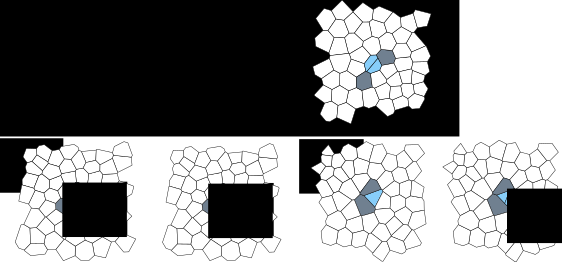
\includegraphics{Figures/division_resolution_figure/division_resolution.pdf}
\caption{Resolving division events. 
Dividing cells are coloured blue. 
(A) Division events are resolved by identifying cells that gain an edge between the time frames (grey cells). 
The dividing cell and the daughter cells are shared neighbours of the grey cells. 
(B) When one of the daughter cells is four-sided, two mother cells are possible, the blue marked mother cell, and the cell marked by an `x'. 
(C) When one of the daughter cells is three-sided the mother cell can be mistaken as having gained an edge if it is identified with the daughter cell marked by an `x'. 
Our algorithm correctly resolves division events such as in (A), (B), and (C).}
\label{fig:division_resolution}
\end{figure}

%%%%%%%%%%%%%%%%%%%%%%%%%%%%

For each $M'$, we define $S_{M,1} = \psi^{-1}_n(\Gamma_G'(M'))$ to be the set of inverse images of the mapped neighbours of $M'$ under $\psi_{n}$. 
Next, we identify the set $S_{\mathrm{border}} \subseteq S_{M,1}$ of potential bordering cells of the division, i.e. cells that are adjacent to the division, by finding those vertices $v \in S_{M,1}$ that gain an edge under the tracking mapping $\psi_{n}$:
%
\begin{equation}
S_{\mathrm{border}} = \{ v \in S_{M,1} : p_{G'}(\psi_{n}(v)) = p_{G}(v) + 1 \}.
\end{equation}
%
We also identify the set $S_{\mathrm{mother}}$ of potential mother cells by finding any shared neighbours of potential bordering cells:
%
\begin{equation}
S_{\mathrm{mother}} = \bigcap_{v \in S_{\mathrm{border}}} \Gamma_G(v).
\end{equation}
%
Based on the sets $S_{\mathrm{border}}$ and $S_{\mathrm{mother}}$ we decide which cells are the mother and daughter cells of the division event, distinguishing between the following cases:

\begin{enumerate}[noitemsep,label=(\roman*)]
\item If $S_{\mathrm{mother}}$ contains exactly one vertex, then this is identified as the mother cell of the division, and $M'$ must contain exactly two vertices, which are identified as the daughter cells. 
In this case, neither the mother nor daughter cells are three- or four-sided. 

\item If $S_{\mathrm{mother}} = \emptyset$, then one of the daughter cells must be three-sided (figure~\ref{fig:division_resolution}c). 
In this case, a geometry-inferred selection of mother and daughter cells is required. 
To this end, we define a set of potential daughter cells
%
\begin{equation}
S_{\mathrm{daughter}}' = \psi_{n} (S_{\mathrm{border}}) \bigcup \left( \bigcap_{v' \in \psi_{n} ( S_{\mathrm{border}}) } \Gamma_{G'}(v') \right).
\end{equation}
%
that contains the images of the potential bordering cells and all shared neighbours of these images in $V'$. 
Next, we find a definite daughter cell as an element $v' \in S_{\mathrm{daughter}}$ that is three-sided ($p_{G'}(v) = 3$). 
The geometry-inferred selection of the second daughter cell proceeds as follows. 
For each $w' \in S_{\mathrm{daughter}}' \setminus \{ v' \}$, we construct the \textit{geometrically merged cell} of $v'$ and $w'$ by removing the edge between the polygons that corresponds to $v'$ and $w'$ in the segmentation of the microscopy video frame from which the graph $G'$ was generated, as well as the cell junctions where three or more cells meet at the end of this edge. 
We then calculate the distance of the centroid of the geometrically merged cell to the centroid of the cell associated with vertex $\psi^{-1}_{n}(w')$.
The vertex $w'$ for which this distance is minimal is identified as the second daughter cell, and the mother cell is identified as its inverse image under $\psi_{n}$.

\item If $S_{\mathrm{mother}}$ contains more than one vertex, then we define a set of potential daughter cells as any shared neighbours of images of the potential bordering cells
%
\begin{equation}
S_{\mathrm{daughter}}' = \bigcap_{v' \in \psi_{n} (S_{\mathrm{border}})} \Gamma_{G'}(v').
\end{equation}
%
If $S_{\mathrm{daughter}}'$ contains exactly four vertices, then the mother cell and both daughter cells are four-sided, and the mother cell can be identified as the single vertex in the set $S_{M,2}$, which we define as the set of cells which are shared neighbours of all cells in $S_{M,1}$ (the inverse images of neighbours of the division), and which are not in the domain of $\psi_{n}$, i.e. 
%
\begin{equation}
S_{M,2} = \bigcap_{v \in S_{M,1}}\Gamma_G(v)\setminus \tilde{V}_{n}
\end{equation}
%
The daughter cells correspond to the only two vertices in $M'$. 

If $S_{\mathrm{daughter}}'$ contains exactly three vertices, then one of the daughter cells is four-sided, and we identify this cell as the definite daughter cell of the division $v'$, i.e. we identify $v' \in S_{\mathrm{daughter}}' : p_{G'}(v') = 4$. 
In this case, geometry-inferred selection of the second daughter cell is required, and we achieve this in a similar way to that described for three-sided daughter cells above. 
For each cell $w' \in S_{\mathrm{daughter}}' \setminus \{ v' \}$, we construct the merged cell of $v'$ and $w'$, and calculate the distance of its centroid to the centroid of $\psi_{n}^{-1}(w')$. 
The cell $w' \in S_{\mathrm{daughter}}' \setminus \{ v' \}$ for which this distance is smallest is the second daughter cell.  
Since in this case $S_{mother}$ contains more than one cell, $S_{\mathrm{daughter}}'$ must contain at least three cells\footnote{If $S_{\mathrm{daughter}}'$ contains more than four cells, then our algorithm fails; however, this was never encountered in our test cases.}.
\end{enumerate}

Once each set $M'$ has been inspected and the associated division event has been resolved by identifying the mother and daughter cells, we construct a tracking mapping in which any incorrectly tracked mother cells are removed. 
To this end, we define the set of all mother cells for which geometry-inferred selection has been used as $S_\mathrm{geo}$, and we construct a final tracking mapping $\psi_\mathrm{track}: \tilde{V}_{n} \setminus S_\mathrm{geo} \rightarrow \tilde{V}_{n}' \setminus \psi_{n}(S_\mathrm{geo})$ such that $\psi_\mathrm{track}(v) = \psi_{n}(v)~\forall v \in \tilde{V}_{n}\setminus \psi_n(S_\mathrm{geo})$.

In general, the division resolution step may incorrectly track cells in cases where there is a cell neighbour exchange next to the division, or if there are two adjacent divisions between frames. 
For example, if each of the bordering cells, i.e. the cells adjacent to the division, were to undergo a neighbour exchange in which they lose an edge between images, then our algorithm would fail to correctly resolve the division event. 

\paragraph{Resolving remaining events} 

At this stage, the tracking algorithm for the two consecutive time frames is completed, and it is straightforward to identify cell neighbour exchanges by finding any cells that have changed their polygon number from one frame to the next. 
Cell removal events correspond to any vertices $v \in V$ that are not in the domain of $\psi_\mathrm{track}$, and for which $\Gamma_G(v) \subseteq V_\mathrm{track}$, and that do not correspond to mother cells of a division event.

%%%%%%%%%%%%%%%%%%%%%%%%%%%%%%%%%%%%%%%%%%%%%%%%%%%%%%%%%%%%%%%%%

\subsection*{Computational implementation}

We use Krissinel's MCS finding algorithm \cite{Krissinel2004} to find all RLMs and LMs in the above steps. This algorithm will always halt eventually. 
In particular, since the domains on which the RLMs and LMs are calculated only contain extended neighbourhoods of individual cells, the MCS finding does not pose computational barriers.
We adapt the procedure for MCS finding proposed in \cite{Krissinel2004} in two ways:
(i) whenever a next vertex is considered for mapping, we pick a vertex that is adjacent to already mapped cells, hence the adapted algorithm only finds connected subgraphs;
(ii) since the RLMs and LMs are small, we do not implement subgraph-size dependent conditions to interrupt the search early.

When finding the initial mapping, for any two possible matches LMs are first calculated by considering nearest neighbours only rather than extended neighbourhoods. 
Once the neighbourhoods\footnote{The set of adjacent vertices, $\Gamma_{G}(v) = \{w \in V : \{v, w \} \in E \}$ is called the \textit{neighbourhood} of $v$, so the degree of $v$ is $|\Gamma_{G}(v)|$.
We define the neighbourhood of a subset $V' \subseteq V$ to be $\Gamma_{G}(V') = \{w \in V \setminus V' : \exists \, v \in V' \text{ with } d(w,v) = 1 \}$.} of two matching vertices are found to be isomorphic, the extended neighbourhood is considered. 
This step reduces the time that is needed to find the initial match.

In the computational implementation of the tracking algorithm we use a further vertex-label $c_{G} : V \rightarrow \mathbb{N}$, which we call the \textit{cell identifier}. 
In practice, integer identifiers for a given vertex $v$ arise naturally in the segmentation step. 
Cell identifiers allow us to easily identify vertices and relate them to a cell in a given image independent of how they are stored in the graph structure. 

%Throughout, our implementation makes use of the concept of a vertex matching matrix introduced in \cite{Krissinel2004} to index which vertices are mappable onto each other.
%We store only one copy of the vertex matching matrix in memory in order to minimise the memory footprint of the application, and whenever the MCS construction yields a new vertex matching, this copy of the vertex matching matrix is updated.
%When searching for RLMs and LMs, reduced versions of the vertex matching matrix are created since only small, local subgraphs are analysed.

The code used in this article is publicly available under the 3-clause BSD license as the \mbox{MCSTracker} project (\texttt{https://github.com/kursawe/MCSTracker}). The project is implemented in pure-Python, employs unit-testing \cite{Osborne2014} and is fully documented. Graphs in our code are represented using the NetworkX package in Python \cite{Hagberg2008}.

%%%%%%%%%%%%%%%%%%%%%%%%%%%%%%%%%%%%%%%%%%%%%%%%%%%%%%%%%%%%%%%%%

\subsection*{Generation of \insilico data sets}

To test the algorithm, we generate \insilico data sets that include examples of cell divisions, removals and neighbour exchanges, as well as tissue movement.  
These data sets are generated using Voronoi tessellations modified using Lloyd's relaxation, which resemble cell packings in a variety of epithelial tissues~\cite{Sanchez-Gutierrez2015, Honda1978}.

To generate polygonal patterns of size $m\times n$, where $m$ and $n$ are natural numbers, $(m+g)\times(n+g)$ Voronoi seeds are uniformly random distributed in a 2D domain $\Omega$ of width $m+g$ and height $n+g$ (figure~\ref{fig:lloyds_relaxation}A). 
Here, $g$ is the size of a boundary region that is introduced to reduce the impact of the Voronoi boundary on the patterns. 
The domain $\Omega$ is surrounded by two rows of evenly spaced additional seeds on each side. The inner row has a distance of 0.5 to $\Omega$, and the seed-spacing is 1.0. 
The outer row has a distance of 1.5 to $\Omega$, and the seeds are shifted parallel to the first row by a distance of 0.5. 
The Voronoi tessellation of all these seeds is then constructed. 

%%%%%%%%%%%%%%%%%%%%%%%%%%%%

\begin{figure}[t]
\centering
\includegraphics{Figures/Lloyds_relaxation_figure/Lloyds_relaxation.pdf}
\caption{Generation of \insilico data. 
(A) Random seeds (black dots) are placed inside a domain $\Omega$, the border of which is shown using a black line. 
Additional, evenly spaced seeds are placed outside $\Omega$. 
The Voronoi tessellation of all seeds is shown in grey, excluding Voronoi regions corresponding to the outermost row of seeds, since these are large or unbounded. 
The centroids of the Voronoi regions differ from the seeds, and are shown as grey crosses. 
(B) The centroids of the Voronoi regions in (A) are used as seeds for a new Voronoi tessellation, for which evenly spaced seeds are again added outside the domain $\Omega$. 
Voronoi regions whose centroids lie within a window (dashed black line) at the centre of the domain are collected to form the \insilico tissue (blue). In this figure, one Lloyd's relaxation step ($n_L=1$) is shown. 
Throughout this study, we generate \insilico tissues using $n_L=4$ Lloyd's relaxation steps.}
\label{fig:lloyds_relaxation}
\end{figure}
%%%%%%%%%%%%%%%%%%%%%%%%%%%%

In each Lloyd's relaxation step, the polygons (or infinitely large areas) corresponding to the regularly spaced seeds outside $\Omega$ are removed from the tessellation. Next, the centroid of each remaining polygon is calculated and registered as a new seed. Further seeds are added that again correspond to two rows of evenly spaced seeds outside $\Omega$. 
A new Voronoi tessellation is then constructed (figure~\ref{fig:lloyds_relaxation}B). 
This procedure is repeated for $L$ relaxation steps, after which all generated polygons are discarded except those whose centroid lies within an area occupying $n\times m$ area units in the centre of $\Omega$ (figure~\ref{fig:lloyds_relaxation}B). 

The polygonal tessellations have approximately $m\times n$ polygons of average area 1.0. 
During the generation of the tessellations, evenly spaced seeds outside $\Omega$ are added to prevent the occurrence of infinitely large polygons inside $\Omega$. 
The boundary of size $g$ is added in between the generated tessellation and the evenly spaced seeds in order to reduce the effect of the evenly spaced boundary seeds on the tessellation. Throughout this study, we use $g=8$ and $n_L=4$, resulting in cell packings similar to those observed in the \Drosophila wing imaginal disc~\cite{Sanchez-Gutierrez2015}. We provide further details of how tissue rearrangements are implemented in the Results section. 

\subsection*{Experimental methods}

Live-imaging of cell proliferation was performed in stage-eleven \Drosophila embryos expressing a tagged version of DE-Cadherin (DE-Cadherin::GFP) using a spinning disc confocal microscope, as described in \cite{Narciso2015}. For the embryo setup, a modified version of the standard live-imaging protocol was used \cite{Parton2010}.

%%%%%%%%%%%%%%%%%%%%%%%%%%%%%%%%%%%%%%%%%%%%%%%%%%%%%%%%%%%%%%%%%\\

\paragraph{Data segmentation}

Microscopy images were segmented manually using Seed\-Wa\-ter\-Seg\-men\-ter~\cite{Mashburn2012}. 
Each segmentation was saved as a 16-bit grayscale image where pixels belonging to different cells have different integer values. 
Polygonal tessellations for the tracking algorithm were generated from the segmented image in two steps. 
First, all junctions between three or more cells were identified as points where pixels of three or more different cells meet, and second, vertices were assigned to cells. 
Finally, edges shorter than two pixels (0.5 \textmu m) were removed and replaced by a single vertex at the midpoint of the edge.

%%%%%%%%%%%%%%%%%%%%%%%%%%%%%%%%%%%%%%%%%%%%%%%%%%%%%%%%%%%%%%%%%%
%%%%%%%%%%%%%%%%%%%%%%%%%%%%%%%%%%%%%%%%%%%%%%%%%%%%%%%%%%%%%%%%%%

\section{Results} \label{sec:results}

\paragraph{\textit{In silico} testing of the algorithm.}

To assess the performance of the algorithm, we begin by applying it to \insilico data sets that include cell neighbour exchanges, tissue movement, cell removal and cell division, respectively. In each case, we compare the outcome of the tracking algorithm to the ground truth.

We begin by assessing the ability of the algorithm to resolve permutations in otherwise identical tissues (figure~\ref{fig:mcs}A). 
In this test, a random tessellation of size nine by nine cells is created as described in the Methods section, and integer identifiers $c_i$ are assigned to each cell.
%The random tessellation creates tissues of nine cells wide by nine cells high. 
Next, an identical copy of the tissue is created in which the integer identifiers are randomly shuffled. A ground truth mapping from the first to the second integer identifiers is generated. Next, the algorithm is applied. 
Upon conducting 100 such tests, all identified cell-to-cell mappings are matched correctly, as compared to the ground truth. 
In rare examples, isolated cells at the boundary of the tissue are are not tracked. In these examples, either a single cell has only one adjacent cell in the tissue, or two cells of identical polygon number are adjacent and share exactly one neighbour. 
Neither the MCS detection algorithm, nor the post-processing algorithm are able to resolve such mappings, which involve fewer than four cells in each dataset (fewer than five percent of the tissue). 

%%%%%%%%%%%%%%%%%%%%%%%%%%%%

\begin{figure}[h]
\centering
\includegraphics{Figures/subgraphs_figure/subgraphs_figure.pdf}
\caption{Examples of \insilico test cases. 
In each image, cells identified by the MCS algorithm are highlighted in green (light), whereas cells that have been filled in by the post-processing steps are highlighted in red (dark). 
The algorithm tracks cells between identical tissues (A), in tissues undergoing translation (B), cell neighbour exchange (T1 swap) (C), cell removal (D) and cell division (E).}
\label{fig:mcs}
\end{figure}

%%%%%%%%%%%%%%%%%%%%%%%%%%%%

We design four further tests of tissue rearrangements (figure~\ref{fig:mcs}B-E).
The first test comprises tissue movements between images (figure~\ref{fig:mcs}B). 
In this test, a tissue of size fifteen by eight cells is generated as described in the Methods section. 
Two smaller tissues of width seven are cut out of this tissue, which each cover the full height of the tissue, and which are horizontally translated relative to each other by a distance of two cell lengths. 
The position of each three-cell junction in both tissues is shifted such that the $x$-coordinate of the left-most junction in each tissue is 0.

The second test (figure~\ref{fig:mcs}C) generates cell neighbour exchanges, also called T1 transitions \cite{Nagai1988,Etournay2015}. 
In our implementation of T1 transitions, an edge shared by two cells is replaced by a new perpendicular edge (of length $l_{T1} = 0.2$ units) such that the local cell connectivity changes (figure \ref{fig:methods}B). 
We create two identical copies of a tissue of size nine by nine cells. In the second copy, a T1 transition is performed on an edge in centre of the tissue.

The third test involves cell removal (figure~\ref{fig:mcs}D). 
In this test, we first generate two identical copies of a tissue of size nine by nine cells. 
In the second copy, we replace the central cell by a vertex shared by its neighbouring cells. 
This rearrangement is similar to so-called T2 transitions in the foams literature \cite{Nagai1988}.
The final test involves cell divisions (figure~\ref{fig:mcs}E). 
Here, we once again create two identical copies of size nine by nine cells. 
In the second copy, a cell in the centre of the tissue is divided by introducing a straight line in a random direction through centroid of that cell.

For all tests generated in this way, integer cell identifiers in the second tissue are randomly shuffled, and a ground truth is generated. 
We run 100 realisations of each test case, and compare the tracking outcome to the ground truth. 
In all cases cells are tracked correctly, with at most three unmatched cells at the boundary of the sheet.

In figure~\ref{fig:mcs}, all cells identified after the cleaning step, in which weakly connected cells are removed from the MCS, are coloured green, whereas cells that are identified by the post-processing algorithm are coloured red. 
Note that the exact number of cells that are identified by the post-processing algorithm varies between individual realisations of the tests. 
In many cases, the cells identified by the post-processing algorithm include cells that are adjacent to the cells that are undergoing division, removal or neighbour exchange. 

We next analyse the extent to which the success of our tracking algorithm depends on the number of Lloyd's relaxation steps, $n_{L}$, used to generate the \insilico data sets. 
To investigate this we iteratively increase $n_{L}$, and so generate tissues with increasingly homogeneous graph structures, and repeat all tests.
We find that the algorithm successfully passes all tests for all values of $n_{L}$ from 4 up to 14.

%%%%%%%%%%%%%%%%%%%%%%%%%%%%

\paragraph{Application of the algorithm to \invivo data}

Figure \ref{fig:data_results} shows three sample segmented images of the lateral epidermis of a stage-eleven \Drosophila embryo, taken five minutes apart, and to which we apply the algorithm. 
These images comprise 271, 263 and 263 cells, respectively.
Between the first and the second images, 247 cells are tracked, whereas 245 cells are tracked between the second and third images. 
The number of cells that are tracked across all three images is 234.  
The centroids of cells of previous images are plotted on top of the tracking, showing that the tracking algorithm successfully tracks cells in situations where it is difficult to match cells between images based on the centroid positions alone. 
Cells that include only their corresponding centroid from the previous image are coloured in green, whereas cells that do not include their corresponding centroid from the previous image, and cells that include multiple centroids from the previous image, are coloured in purple. 

%%%%%%%%%%%%%%%%%%%%%%%%%%%%
\begin{figure}[h]
\centering
\includegraphics{Figures/Data_results_figure/Data_results_figure.pdf}
\caption{Three segmented data frames. 
Cells that are tracked across all frames are coloured green or purple, and cells that leave or enter the tissue at the boundary are white. 
Dying cells are black. 
The centroids of tracked cells of the respective previous frames are included as yellow dots, and cells that contain only their centroid from the previous frame are coloured green, whereas cells that do not contain their centroid from the previous frame, and cells that contain multiple centroids, are coloured purple. 
Together, the centroids and the colouring illustrate that it is challenging to track cells between the data frames using solely centroid positions.}
\label{fig:data_results}
\end{figure}

%%%%%%%%%%%%%%%%%%%%%%%%%%%%

On average, cell centroids move 0.75 cell lengths between the first and second images, with a maximal displacement of 1.17 cell lengths. 
Between the first and second images 36 cells undergo a net gain in edges, whereas 20 cells have net loss of edges. 
In total, four cell deaths and no cell divisions are observed across all three data images, and none of the cells are tracked incorrectly. 

%%%%%%%%%%%%%%%%%%%%%%%%%%%%

\paragraph{Calculation times}

To analyse the scaling of the calculation times with tissue size we repeat the permutation test with tissues of square dimension of varying size on a desktop computer with an Intel i5-6500T CPU (2.5GHz) and 8GB R. We find that the calculation times scale subquadratically with cell number (figure~\ref{fig:calculation_times}). 

%%%%%%%%%%%%%%%%%%%%%%%%%%%%
\clearpage
\begin{figure}[h]
\centering
\includegraphics{Figures/Timings_figure/calculation_times.pdf}
\caption{Scaling of the calculation times with tissue size. 
Virtual tissues of square dimension of varying sizes were generated and the calculation times of the algorithm under the permutation test in figure~\ref{fig:mcs}A recorded. 
Orange dots represent calculation times for individual realisations of the test and error bars denote the standard deviation. 
The exponent $b$ of the polynomial fit is 1.6. 
The calculation times were measured on a desktop computer with an Intel i5-6500T CPU (2.5GHz) and 8GB R.}
\label{fig:calculation_times}
\end{figure}

%%%%%%%%%%%%%%%%%%%%%%%%%%%%


The calculation times for the experimental images analysed in figure \ref{fig:data_results} vary more widely than for the \insilico data sets. 
For the tracking between the first and second frames in this figure, the algorithm required 96 seconds to run, whereas between the second and the third frames the algorithm required 15 seconds. 
This difference appears to arise from differences in the time required to find the first correct mapping. 
In the first example 154 cells were searched before the first correct mapping was found, whereas in the second example only 12 cells were searched. This means that the number of cells considered when finding the initial mappings depends on the graph structure of the analysed frames and impacts on the calculation time of the algorithm. 

\paragraph{Algorithm performance on rearranging tissues}

To assess the performance of the algorithm on rearranging tissues, we applied the algorithm to \insilico data sets with increasing numbers of cell rearrangements (figure \ref{fig:t1_analysis}).
The number of correctly tracked cells decreases as the number cell rearrangements increases. However, the number of incorrectly tracked cells remains low even for large numbers of cell rearrangements. 

%%%%%%%%%%%%%%%%%%%%%%%%%%%%
\clearpage
\begin{figure}[h]
\centering
\includegraphics{Figures/T1_swap_figure/t1_swap_analysis_full.pdf}
\caption{Success rate of the algorithm on \insilico tissues with increasing amounts of cell rearrangements. 
Virtual tissues spanning 20 cell lengths in each dimension are generated, and T1 swaps are applied to an increasing proportion of the inner edges of the tissue.
For each ratio of T1 swaps, 10 repetitions of the test are run, and the ratio of correctly and incorrectly tracked cells in the tissue is recorded.
The dashed blue and solid red lines correspond to mean values of correctly and incorrectly tracked cells, respectively. Error bars denote the standard deviation of the mean, and results of individual runs of the test are represented by dots.}
\label{fig:t1_analysis}
\end{figure}

%%%%%%%%%%%%%%%%%%%%%%%%%%%%



The number of untracked cells increases rapidly as the percentage of edge rearrangements, i.e. the percentage of inner edges in the tissue that are swapped between successive images, increases from five to ten percent.
Note that the number of cells involved in these cell rearrangements is larger than five to ten percent, since an individual T1 transition changes the cell neighbour relations of four different cells, and each cell shares multiple inner edges.
For example, rearranging five percent of the inner edges of the tissue affects roughly 40 percent of the cells in the tissue, whereas rearranging ten percent of the tissue edges affects up to 70 percent of the cells. 
The number of (correctly or incorrectly) tracked cells drops to zero if the tissue rearranges so much that the extended neighbourhood of each cell rearranges. In this case a first match cannot be found to initialise the MCS construction algorithm.

%%%%%%%%%%%%%%%%%%%%%%%%%%%%%%%%%%%%%%%%%%%%%%%%%%%%%%%%%%%%%%%%%%
%%%%%%%%%%%%%%%%%%%%%%%%%%%%%%%%%%%%%%%%%%%%%%%%%%%%%%%%%%%%%%%%%%

\section{Discussion} \label{sec:discussion}

Cell tracking in epithelial sheets has the potential to generate a vast amount of quantitative data to inform our understanding of the contributions of different cellular processes to tissue morphogenesis. 
However, cell tracking is notoriously difficult, especially for the complex morphogenetic processes that occur as embryogenesis proceeds.
Here, we present an algorithm based on MCS detection for the tracking of cells in segmented images of epithelial sheets. 
Our algorithm successfully tracks cells in \invivo images of the \Drosophila embryonic epidermis, as well as in randomly generated \insilico data sets, without the need for the adjustment of tissue specific parameters, such as weights for individual terms in a global minimisation scheme \cite{Padfield2011}. 
The use of \insilico data to test our algorithm allows us to analyse the performance of our algorithm for a large range of experimentally observed cell rearrangements and tessellations. 

Our algorithm is able to track cells that undergo significant movement and neighbour exchanges between frames. 
For example, we can correctly track cells in tissues where more than 40 percent of the cells rearrange between successive movie frames (figure \ref{fig:t1_analysis}).
In addition, even comparably large gaps in the initial MCS can be filled in during the post-processing step (figures \ref{fig:methods} and \ref{fig:data_results}). 
For example, in the first tracking step in figure \ref{fig:data}, only 182 of the 246 tracked cells were identified by the MCS algorithm, and it was possible to track the 64 remaining cells during the post-processing step.  
For comparison, Heller et al \cite{Heller2016} report 15 cell rearrangements per 1000 cells per hour at an imaging interval of six minutes for their time-laps microscopy data of \Drosophila wing imaginal discs.
In addition, the experimental data shown in figures \ref{fig:methods} and \ref{fig:data_results}, as well as our \insilico cell removal data sets, contain multicellular rosettes, hence rosettes do not pose a challenge to our algorithm.

Our algorithm is able to correctly track cells in all considered test cases. However, on rare occasions a few cells at the tissue boundary cannot be tracked. 
It may be possible to adapt the algorithm to track these cells, if this is considered necessary for the application at hand. 
In the current version of the algorithm, two connections to already tracked cells that are preserved between two time frames are a condition to add a cell-to-cell mapping in the post-processing algorithm. 
Further analysis of cases where this condition is not fulfilled may reveal ways to relax it.

When generating \insilico data to test the algorithm, we used Voronoi tessellations in combination with Lloyd's relaxation to generate data that resembles tissues in the \Drosophila wing imaginal disc \cite{Sanchez-Gutierrez2015}.
We expect the algorithm to perform less well on tissues whose network structure is near homogeneous.
For example, in an epithelial sheet where cells are arranged in a hexagonal fashion, such as the early \Drosophila embryonic epidermis \cite{Warn1983} or the late pupal \Drosophila wing \cite{Classen2005}, the local adjacency network of each cell is identical, and hence a network-based tracking algorithm may not be able to distinguish cells.
When generating \insilico tissues, we use four Lloyd's relaxation steps after Voronoi tessellation.
With each Lloyd's relaxation step, the homogeneity of the tissue increases.
We were able to successfully repeat all \insilico tests on virtual tissues that were generated using up to $n_L=14$ Lloyd's relaxation steps.
Hence, we expect the algorithm to be suitable for tissues that can be well described with 14 or fewer Lloyd's relaxation steps, such as the chick neural tube embryonic epithelium, or the \Drosophila eye disc \cite{Sanchez-Gutierrez2015}.

The algorithm relies on being able to generate polygonal tessellations from segmented video microscopy data. 
In particular, all \insilico tests we conducted consider tissues where each cell has at least three neighbours. Conceptually, it would be possible to apply the algorithm to tissues in which individual cells may have only two neighbours, although such examples have not been included in our analysis.

In microscopy videos including division events we expect the algorithm to perform well in tissues in which no adjacent divisions occur between successive movie frames, and in which cells adjacent to the dividing cell do not undergo rearrangements before the next frame is captured. 
Our algorithm is designed to identify mother and daughter cells of a division event by establishing which are the bordering cells that gain an edge during the division event. 
In the case of two adjacent divisions, and if cells adjacent to a division event gain edges due to cell rearrangements, the dividing cell cannot be correctly identified.
An example of a typical tracking error for two adjacent divisions is shown in figure \ref{fig:adjacent_divisions}. 
In cases where the division resolution step fails, our Python implementation returns all tracked cells of the post-processing step, and gives a warning that the division has not been resolved. 
In these cases, manual correction methods could be used for incorrectly tracked cells in the vicinity of division events.

%%%%%%%%%%%%%%%%%%%%%%%%%%%%
\begin{figure}[h!]
\centering
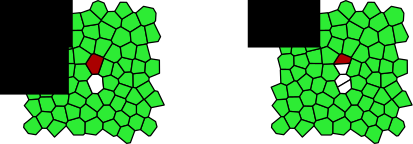
\includegraphics{Figures/double_division_figure/double_division_figure.pdf}
\caption{Tracking errors can occur if adjacent cells divide. Here, all green (light) cells are tracked correctly. One of the mother cells (red/dark) of the division events has been incorrectly associated with one of the daughter cells of the division.}
\label{fig:adjacent_divisions}
\end{figure}

%%%%%%%%%%%%%%%%%%%%%%%%%%%%

The parameters of the algorithm are chosen to maximise the robustness of the algorithm and avoid the necessity to adjust the parameters to individual applications.
For example, the cutoff length, $d_{\mathrm{max}}$, that determines the distance below which two cells in consecutive movie frames are considered mappable to each other was chosen at 10 times the average cell length in the tissue, which is significantly larger than the movement that is to be expected between consecutive frames of a live-imaging microscopy video.
However, parameter adjustments may be possible for individual applications in order to decrease the algorithm calculation times.
For example, the size of the extended neighbourhood considered in the initial step or the iterative extension could be reduced to include only nearest neighbours instead of nearest neighbours and second nearest neighbours in case the tissue is sufficiently heterogeneous.
Similarly, one might decrease the cutoff length, $d_\mathrm{max}$, for possible cell pairings if the cell positions are not expected to vary significantly between time frames. 
When filling in any gaps in the MCS (figure~\ref{fig:methods}C-D), requiring that $n_{p} = 4$ neighbours are preserved between consecutive frames for newly added cells seems to be a sufficiently large number in practice. 
However, it is possible to start the post-processing requiring a higher number of previously mapped neighbours for the tracking.

Adjustments may be possible to extend the applicability of the algorithm to a wider range of tissues. 
For example, instead of automatic detection of the initial seeds for the MCS detection algorithm, a small set of seeds could be manually supplied to guide the tracking. 
This should improve the performance of the algorithm on homogeneous tissues. 
A further option to improve tracking of cells in homogeneous tissues is to make adaptations that ensure that the cyclic order of neighbours of each cell is preserved under the mapping. 
In such cases, irregular boundaries may also help to aid the initial seeding. 
Finally, in cases where the algorithm is not able to track all cells due to a larger number of cell neighbour exchanges than in the tissues considered here, it may be possible to extend the current algorithm by removing the assumption that the MCS is connected, and using a set of non-adjacent cells as initial seeds.

In the presented work, we have deliberately kept the geometrical input to the algorithm to a minimum. 
Cases where geometric data are taken into account comprise division events where one of the daughter cells is four- or three- sided, since in these cases we are not able to make a decision on which cell is the second daughter cell based on network adjacency alone. 
If future applications reveal cases where the algorithm performs poorly due to a large number of cell neighbour exchanges or high degree of tissue homogeneity, it may be possible to construct algorithms that combine information on the network topology with data on cell shapes, cell positions and cell movements to improve performance. For example, information on network topology could be integrated into previous algorithms which minimise differences between geometric properties of cells, such as cell size and location~\cite{Puliafito2012}, with information about network connectivity. 

In cell tracking applications, the scaling of the algorithm with tissue size is crucial. 
Potential applications range from systems of 30 cells (\Drosophila embryonic epidermal P compartments \cite{Parker2006}), to 10,000 cells (\Drosophila imaginal wing disc \cite{Farhadifar2007}). 
Calculation times in the presented algorithm scale subquadratically with cell number, making it suitable for applications of varying sizes. 
For example, extrapolating the data in figure \ref{fig:calculation_times}, a tissue of 10,000 cells could be tracked across two frames within 20 minutes. The scaling of the algorithm is polynomial despite the fact that it is based on MCS detection, which is known to be an NP-hard problem in the general case, i.e. the calculation times scale exponentially with the problem size. 
MCS detection has a wide range of research applications, including protein interaction networks~\cite{Ciriello2012, Aladag2013} and finding the binding sites of chemical structures~\cite{Raymond2002}. 
Our approach of reducing the MCS search to a local, close to quadratically scaling search may have applications in other areas where the networks are inherently planar.

Our algorithm is designed to track cells in segmented microscopy videos of epithelial sheets in two dimensions. However, it may be possible to apply the algorithm to datasets of epithelial sheets that are embedded in a three-dimensional environment, such as the \Drosophila imaginal wing disc~\cite{Mao2011}, or the \Drosophila embryonic epidermis~\cite{Parker2006, Rauzi2008}, including tissues that can be mapped onto a cylinder or ellipsoid, such as the mouse visceral endoderm \cite{Trichas2012}. 

A large number of cell tracking algorithms have been developed for varying applications~\cite{Mashburn2012, Cilla2015, Padfield2011, Youssef2011,Schiegg2013,Heller2016,Liu2014,Raffel2007,Kofahi2010,Amat2014,Wait2014, Winter2011, Sommer2011, Bellaiche2011, Aly2014, Wang2010, Puliafito2012, Aigouy2010}. 
Further efforts are required to compare these algorithms with our own, and to identify the algorithm best suited for an individual data set. 
In the cell tracking challenge \cite{Maska2014} the authors provide microscopy videos from a variety of \invitro cell cultures, including, for example, mouse embryonic stem cells and human squamous lung carcinoma cells, together with ground-truth segmentation and tracking data as benchmarks for cell tracking and segmentation algorithms. 
However, many of the published algorithms above have not yet been applied to the challenge, and benchmark datasets for epithelial sheets are currently not available. 
In~\cite{Chenouard2014} \insilico data sets are used as benchmarking data sets for particle tracking algorithms.

The proposed algorithm provides a tracking solution specialised for cell-tracking in epithelial sheets that attempts to maximise the information that can be gained from the packing that is typical to epithelial tissues. 
It may, however, be possible to extend this algorithm to applications of two-dimensional cell tracking where cells are not physically connected by constructing adjacency networks from Voronoi tessellations that use the cell locations as seeds.  
We hope that, as segmentation tools are developed further, the combination of our algorithm with these tools will lead to further insights into cellular behaviour in epithelial tissues.

%%%%%%%%%%%%%%%%%%%%%%%%%%%%

%\paragraph{Other comments and questions}

%\begin{itemize}[noitemsep]
%\item Somewhere in the discussion, we should refer to issues associated with performing cell tracking (with our method, and others) on curved (non-planar) epithelial cell sheets. \jochen{The discussion mentions that this would be possible. What are the issues that we should be addressing here?}
%\item Somewhere in the results section, I would like to see a breakdown of the proportion of time spent in each part of the algorithm (initial identification of MCS and each post-processing step) when it is applied to an example. \jochen{We do this at the end of the results section already, under `calculation times'. I leave the comment in for now until we generated and added the new results.}
%
%\item I noticed the following things when making the t1 percentage figure 
%\begin{itemize}
%\item When many t1 swaps happen around the same cell, the postprocessing in its current form may go wrong, see figure \ref{fig:t1_example}. 
%I have attempted to adapt the algorithm to enable it to track examples like the one in figure \ref{fig:t1_example}, but this is not yet working. Whether this is necessary depends on how many T1 swaps we really expect in consecutive time frames.
%\item This seems to be the main reason why the number of correctly tracked cells goes down even for small numbers of t1 swaps.
%\item When discussing this (and in order to know whether the algorithm needs to be improved), it would be useful to know how many T1 swaps we would expect between consecutive time frames of a microscopy video. $\rightarrow$ Jeremy's response: Typical numbers: from epitools paper (Heller et al. 2016, 10-15 per 1000 cells per hour for ex vivo cultured 3rd instar wing discs) see figure 7B in the Epitools paper for the graph. There are possible other values from different contexts but let me know if you want more than one reference. The Etournay et al. elife paper from the Eaton lab plots the T1 contribution to tissue shear during pupal wing morphogenesis, but this is a little hard to translate into no. of T1 transitions per cells/per time. If you would like to estimate this, then we can do it for the embryo where there are lots of T1 transitions but we'd need to coordinate with you on applying your algorithm to several example videos. 
%\end{itemize}
%
%\item I started to work on making the same figure as \ref{fig:t1_analysis} in dependence of cell removal rate.
%The problem here is that my code for cell removal cannot yet remove cells that are adjacent to a rosette. This is necessary, since each cell removal creates a rosette, and hence we need to fix it if we want to include adjacent death events. - Comment here you think this figure wouldn't be necessary.
%
%\item consider comparison to Epitools (also: add citation to Epitools), and the min-cost-flow algorithm.
%\item consider performance comparison to manual seedwater adjustment on insilico data. $\rightarrow$ Jeremy's comment: I'm not sure if I understand this bullet point. We are still trying to get Epitools to work in our hands.Cody finds that our matlab implementation of seedwater segmenter is relatively robust to work with to segment individual frames. If you want manually curated videos for your paper or for a future submission, let us know.
%
%\item \alex{Question: What happens if you run your algorithm on a sequence of images that run backward in time? Does it do any better/worse? (I guess this question boils down to whether the algorithm fares better with cell removal or cell division?)} Answer: It sounds like a good idea to to run the algorithm again `backwards' if it were to work better on either cell division or cell death. However, in practice that's not true, since the identification of a cell division event requires an identification of a mother cell and two daughter cells (1 cell $\rightarrow$ 2 cells), whereas the identification of a cell death event simply requires to identify a cell that `has gone missing' (1 cell $\rightarrow$ no cell). Hence, we can not understand cell division as a reverse cell death. To fully answer the question, since it is structurally simpler to resolve a cell death event than a cell division event I would expect the algorithm to perform better on data including cell death rather than cell division. In particular, I believe the algorithm in the current form should be able to resolve adjacent cell death events (again, still trying to implement this), whereas it is not able to deal with adjacent divisions (see comments on this in discussion section).
%$\rightarrow$ Jeremy's comment: Would it help to include the fact that mother cells expand apical areas before divisions? Response: Technically, probably yes. However, in this initial stage of the algorithm we only perform tracking of two consecutive data frames.
%
%\item Jeremy's comments:
%  \begin{itemize}
%    \item should there be an associated overarching workflow diagram illustration that has arrows between each of the steps? Input: voronoi tesselations based on segmented images, bijections, identification of new cells, etc.? $\rightarrow$ Do you mean in addition to Fig \ref{fig:methods}?
%    \item As an aside, I could not follow all of the shorthand and would love to have a conversation/tutorial at a later time to learn some of it (even where there might be a graph terminology for dummies/glossary). For example what is the $\prime$ symbol signify, and $\setminus$.
%    \item There could be multiple maximum common subgraphs? $\rightarrow$ Yes, there can. Our algorithm is designed to find what we call the conserved MCS which includes all cells that are part of each MCS.
%    \item consider providing a reference or definition of unit testing
%    \item How was this (cell division, rearrangement etc.) simulated in the in silico data sets? I realize that this is discussed below but should there also be a summary sentence in methods?
%    \item You can use the limits on cell rearrangements to help calibrate experimental settings and limits on intervals of acquiring time-lapse data 
%    \item Jeremiah Zartman: you could also run your ground-truth in silico data through epitools or packing analyzer for comparison (if asked by the reviewer). If a reviewer asks for this then you can turn it around and claim that the in silico data sets could be used to compare new and alternative cell tracking solutions.
%    \item 20 min of calculation time between a single time frame? $\rightarrow$ Yes. Keep in mind though that this process can be parallelized since the program is sequential, i.e. on a normal workstation/laptop with 4 cores you track up to 4 frames at the same time, on a cluster you could do a lot more than that.
%    \item Jeremiah Zartman: Instead of calling it "this algorithm" do you want to give it a name, like MCS tracker or NetworkTracker or something like that?
%    \item Concerning non-tracked cells at the boundary: It may be sufficient to just highlight "non tracked cells" if it is minimal.
%    \item adjacent divisions problem is potentially problematic for the embryo for clustered division events, but you could work around it by also factoring changes of cell area during rounded cells.
%    \item Jeremiah Zartman: the pouch is more on the order of
%~3000 cells, the whole disc at final larval size is 30-50,000
%cells, but at this level you'd need to be able to handle the
%curvature $\rightarrow$ what would be good references for these numbers?
%    \item Not related to this manuscript, but questions I have: Should we be generating these benchmark datasets? I'd be open to having conversations on this. What sort of criteria or qualities would go into such a benchmark dataset? Would generation of bench mark in vivo data set plus initial comparison be a good follow-up study?
%    \item concerning application of the algorithm to 2D data without connectivity: In biology terminology, do you mean subconfluent epithelial cell culture or wound healing applications? $\rightarrow$ Does subconfluent mean the cells don't adhere to each other and form connections? In this case: Yes. Why do wound healing applications fit into this category?
%    \item adjacent cell divisions happen frequently in the embryo. How does the algorithm handle \invivo data with prominent mitotic rounding.
%    \item Figure 2A gap at the top: is this several cell divisions in a cluster?
%    \end{itemize}
%\end{itemize}

%%%%%%%%%%%%%%%%%%%%%%%%%%%%%%%%%%%%%%%%%%%%%%%%%%%%%%%%%%%%%%%%%%
%%%%%%%%%%%%%%%%%%%%%%%%%%%%%%%%%%%%%%%%%%%%%%%%%%%%%%%%%%%%%%%%%%

\section*{Acknowledgements}

J.K. acknowledges funding from the Engineering and Physical Sciences Research Council through a studentship. J.Z. acknowledges funding support from the National Science Foundation (awards CBET-1553826 and CBET- 1403887). The authors thank Cody Narciso for sharing the microscopy data.

%%%%%%%%%%%%%%%%%%%%%%%%%%%%%%%%%%%%%%%%%%%%%%%%%%%%%%%%%%%%%%%%%%
%%%%%%%%%%%%%%%%%%%%%%%%%%%%%%%%%%%%%%%%%%%%%%%%%%%%%%%%%%%%%%%%%%

\bibliographystyle{royalsociety.bst}
\bibliography{library.bib}

%%%%%%%%%%%%%%%%%%%%%%%%%%%%%%%%%%%%%%%%%%%%%%%%%%%%%%%%%%%%%%%%%%
%%%%%%%%%%%%%%%%%%%%%%%%%%%%%%%%%%%%%%%%%%%%%%%%%%%%%%%%%%%%%%%%%%

\clearpage
%\section*{Figures and captions}

%\begin{figure}[h!]
%\centering
%\includegraphics{cell_network_figure.pdf}
%\caption{Overlay of a polygonal tessellation (grey) and the corresponding cell network (black). Each cell corresponds to one vertex in the network, and two vertices share an edge if the corresponding cells are adjacent. The network of cells is used by the algorithm to determine the MCS between tessellations corresponding consecutive time frames in a microscopy video. Note that the network degree of a cell and its polygon number differ at the boundary of the tissue. \todo{merge this figure with Fig1 or Fig4}}
%\label{fig:cell_network}
%\end{figure}

%\begin{figure}[ht!]
%\centering
%\includegraphics[scale=1.2]{multiple_t1_example_3_after.pdf}
%\includegraphics[scale=1.2]{multiple_t1_example_3_before.pdf}
%\caption{Example of an incorrectly tracked cell. FOR DISCUSSION ONLY, not part of the manuscript. The cell that has been tracked incorrectly next to the gap underwent multiple rearrangements between the consecutive time frames, and that is why the algorithm struggles to track it correctly.}
%\label{fig:t1_example}
%\end{figure}

%%%%%%%%%%%%%%%%%%%%%%%%%%%%%%%%%%%%%%%%%%%%%%%%%%%%%%%%%%%%%%%%%%
%%%%%%%%%%%%%%%%%%%%%%%%%%%%%%%%%%%%%%%%%%%%%%%%%%%%%%%%%%%%%%%%%%

\end{document}
